\documentclass[12pt,twoside, a4paper, twocolumn]{article}
\usepackage[utf8]{inputenc}
\usepackage[brazil]{babel}
\usepackage[margin = 0.5in]{geometry}
\usepackage{amsmath}
\usepackage{amsthm}
\usepackage{amssymb}
\usepackage{amsthm}
\usepackage{setspace}
\usepackage[americanvoltages,fulldiodes,siunitx]{circuitikz}
\usepackage{lipsum}
\usepackage{pgfplots}
\usepackage{ifthen}
\usepackage{adjustbox}
\usepackage[section]{placeins}
\usepackage{hyperref}
\usepackage{graphicx}
\usepackage{adjustbox}
\pgfplotsset{compat=newest}
\graphicspath{ {./images/} }
%  #1 color - optional #2 x_0 #3 y_0 #4 x_f #5 y_f #6 name - optional  #7 true if adding lines to axis
\newcommand{\drawvector} [9] [color=cyan] {
\draw[line width=1.5pt,#1,-stealth](axis cs: #2, #3)--(axis cs: #4, #5) node[anchor=south west]{$#6$};
\ifthenelse{\equal{#7}{true}}{
\draw[line width=1pt,#1, dashed](axis cs: #4, #5)--(axis cs: #4, 0) node[anchor= north west]{$#8$};
\draw[line width=1pt,#1, dashed](axis cs: #4, #5)--(axis cs: 0, #5) node[anchor=south east]{$#9$};
}
{}
}
\newcommand\deriv[2]{\frac{\mathrm d #1}{\mathrm d #2}}
\title{Decimo  Relatório de Física Experimental 2}
\author{Henrique da Silva \\ hpsilva@proton.me}
\date{\today}
\pgfplotsset{width = 10cm, compat = 1.9}
\begin{document}
\maketitle
\pagenumbering{gobble}
\newpage
%pagenumbering{roman}
\tableofcontents
\newpage

\section{Introdução}

\paragraph*{Neste relatório, vamos discutir difracao de fendas simples, redes de difracao, e decomposicao espectral.}

\paragraph*{Também discutiremos alguns circuitos retificadores com diodos.}

\paragraph*{Todos arquivos utilizados para criar este relatório, é o relatório em si estão em:  \url{https://github.com/Shapis/ufpe_ee/tree/main/4th semester/}}


\section{Difracao de Fraunhofer}


\subsection{Tabela de dados inicial}

\begin{center}
  \begin{tabular}{ |c|c|c| }
    \hline
    $Paquimetro$          & $Primeiro\,Minimo$    \\
    $(0.10 \pm 0.05)\,mm$ & $(1.55 \pm 0.05)\,cm$ \\
    $(0.20 \pm 0.05)\,mm$ & $(1.15 \pm 0.05)\,cm$ \\
    $(0.30 \pm 0.05)\,mm$ & $(0.50 \pm 0.05)\,cm$ \\
    $(0.40 \pm 0.05)\,mm$ & $(0.40 \pm 0.05)\,cm$ \\
    $(0.50 \pm 0.05)\,mm$ & $(0.35 \pm 0.05)\,cm$ \\
    \hline
  \end{tabular}
\end{center}


\subsection{Analise Teorica}
\subparagraph*{Para prosseguirmos precisamos lembrar das seguintes relacoes:}

\begin{equation}
  \begin{aligned}
     & a * \sin \theta = m \lambda     \\
     & m = 1                           \\
     & a * \sin \theta = \lambda       \\
     & \sin \theta = \frac{\lambda}{a} \\
  \end{aligned}
\end{equation}

\subparagraph*{Que nos da uma relacao linear se consideramos ao inves de $a$, consideramos seu inverso $\gamma = 1/a$.}

\begin{equation}
  \sin \theta = \lambda \gamma
\end{equation}


\subsection{Tabela de dados extendida}
\begin{center}
  \begin{tabular}{ |c|c|c|c|c| }
    \hline
    $a$                   & $1/a$                 & $y$                   & $x$             & $\sin{\theta}$        \\
    $(0.10 \pm 0.05)\,mm$ & $(10.0 \pm 2)mm^{-1}$ & $(1.55 \pm 0.05)\,cm$ & $(217 \pm 5)cm$ & $(0.0071 \pm 0.0005)$ \\
    $(0.20 \pm 0.05)\,mm$ & $(5.0 \pm 2)mm^{-1}$  & $(1.15 \pm 0.05)\,cm$ & $(217 \pm 5)cm$ & $(0.0053 \pm 0.0005)$ \\
    $(0.30 \pm 0.05)\,mm$ & $(3.3 \pm 2)mm^{-1}$  & $(0.50 \pm 0.05)\,cm$ & $(217 \pm 5)cm$ & $(0.0023 \pm 0.0005)$ \\
    $(0.40 \pm 0.05)\,mm$ & $(2.5 \pm 2)mm^{-1}$  & $(0.40 \pm 0.05)\,cm$ & $(217 \pm 5)cm$ & $(0.0018 \pm 0.0005)$ \\
    $(0.50 \pm 0.05)\,mm$ & $(2.0 \pm 2)mm^{-1}$  & $(0.35 \pm 0.05)\,cm$ & $(217 \pm 5)cm$ & $(0.0016 \pm 0.0005)$ \\
    \hline
  \end{tabular}
\end{center}

\subsection{Grafico de $\sin{\theta}$ vs $1/a$}

\begin{adjustbox}{scale=0.70}
  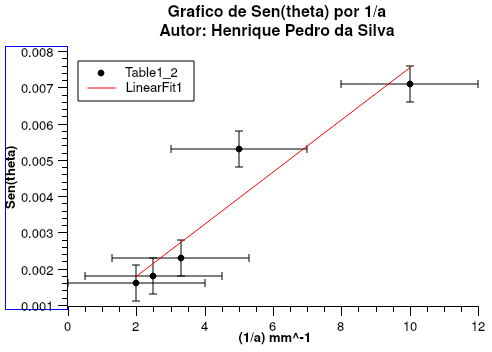
\includegraphics{Graph1.png}
\end{adjustbox}

\subparagraph*{Podemos ver de fato, que como esperado obtemos uma relacao linear entre $\sin{\theta}$ e $1/a$.}

\subparagraph*{E o coeficiente angular da reta, encontrado foi de $717.4$. Porem, com error na ordem de $100$.}

\subparagraph*{Logo podemos afirmar que o comprimento de onda encontrado foi de $700 \pm 100$ nm. Que esta dentro do esperado.}

\subparagraph*{E seu percentual de desvio foi de $10\%$ aproximadamente.}

\pagebreak

\newpage

\subsection{Difracao de objeto microscopico}

\subparagraph*{Nos medimos uma abertura de $3.1cm$ ou seja. Nosso $x$ e $y$ sao os mesmos do caso da abertura de $0.1mm$ do paquimetro.}

\subparagraph*{Logo, convenientemente pelo principio de Babinet podemos reutilizar todos dados que obtivemos para a abertura de $0.1mm$ do paquimero.}

\subparagraph*{E obteremos os seguintes resultados:}

\begin{equation}
  \begin{aligned}
     & a =(0.10 \pm 0.05)\,mm             \\
     & \frac{1}{a} = (10.0 \pm 2)mm^{-1}  \\
     & y = (1.55 \pm 0.05)\,cm            \\
     & x = (217 \pm 5)cm                  \\
     & \sin{\theta} = (0.0071 \pm 0.0005) \\
     & \theta = (0.41 \pm 0.05)\,graus    \\
  \end{aligned}
\end{equation}

\subparagraph*{Podemos tambem simplesmenet usar a relacao:}

\begin{equation}
  a = \frac{\lambda}{\sin{\theta}}
\end{equation}

\subparagraph*{Que nos da: $0.09 \pm 0.02$mm}

\subparagraph*{Que esta dentro do esperado. Ja que a mesma abertura do laser tinha sido observada com o paquimetro aberto em $0.1mm$.}

\newpage

\pagebreak

\section{Redes de difracao}

\subsection{Sistema com rede de difracao conhecida}

\begin{equation}
  Y_1 = (7.15 \pm 0.05)cm
\end{equation}


\subparagraph*{Com a aproximacao $\theta_1 = Y_1/l = (0.358 \pm 0.007)rad$}

\subparagraph*{Utilizando as seguintes relacoes:}

\begin{equation}
  \begin{aligned}
     & d \sin(\theta) = m \lambda \\
     & f = \frac{1}{d}            \\
  \end{aligned}
\end{equation}

\subparagraph*{Temos que $d = (1805 \pm 8) nm$ e $f = (554 \pm 5) \frac{nm}{mm}$ }

\subparagraph*{O valor do fabricante foi de  $540 \frac{nm}{mm}$.}

\subparagraph*{Entao a ordem do erro seria aproximadamente $2\%$.}

\subsection{Sistema utilizando CD como rede de difracao}






\end{document}